\label{sec:4_experiments_and_results}

\begin{comment}
It is important to “verify” your solutions and ideas with an evaluation. This should be described in this chapter.

INTRO: What will you look at in this chapter and why? Again, point back to the summary in the last chapter, and say that here you want to experiment with and evaluate the proposed “solution”.

MIDDLE SECTIONS: Explain your experiments and evaluations. Include a detailed description of the data you have used, and which metrics you include. It is nice to discuss what the results also mean (in general and in the context of your problem statement), not only what you can observe. Also, try to explain WHY the results turn out as they do. You are a researcher and should try to understand why things happen, not only observe what happens.

DISCUSSION: (some put this as a separate chapter before the conclusion depending on the length of it) It is often also nice to discuss the results in a broader setting, trying to generalize the results beyond the specific case study and selected data. This is often done in a separate discussion section at the end - or if it is a lot to discuss, as a separate chapter. Here, one can also typically include a discussion of challenges and pitfalls experienced, etc.

SUMMARY: As above, the summary section should summarize your achievements, results, etc. Briefly conclude what they mean, and what you have learned. NO need to lead to the next chapter - the conclusion.
\end{comment}


% INTRO:



% MIDDLE SECTIONS:

\label{4_investigatory_experiments}

\begin{comment}
INTRO: What will you look at in this chapter and why? Again, point back to the summary in the last chapter, and say that here you want to experiment with and evaluate the proposed “solution”.
\end{comment}



\begin{comment}
MIDDLE SECTIONS: Explain your experiments and evaluations. Include a detailed description of the data you have used, and which metrics you include. It is nice to discuss what the results also mean (in general and in the context of your problem statement), not only what you can observe. Also, try to explain WHY the results turn out as they do. You are a researcher and should try to understand why things happen, not only observe what happens.
\end{comment}

\section{Alpaca on Medical Images\\- Investigatory Experiments}

Before tuning the model on the complete dataset, a subsection of the available training data was used to see how the model would respond. By running the model on smaller training data, it is possible to get initial results faster, which can give insight into where the method could improve. 

    \subsection{5000 samples and 3 epochs}

    The first investigatory experiments were conducted using a subset of the original dataset. The subset was chosen to be on 5000 samples, which correlates to 9,7\% of the total dataset. The reason to do the initial investigatory experiment with this subset is to test the feasibility of the method and implementation, without using unnecessary time and computing resources. 


    To finetune the Stanford Alpaca model, the original authors suggest training for two or three epochs. This is to lot let the model forget the previous knowledge and still be able to use the knowledge gathered from the original training corpus. Therefore, in this run, the hyperparameters were chosen as in Table \ref{table:hyperparameters_5000}. The rationale for deciding on the values for batch size and micro-batch size was to make it fit in the available RAM on the GPU that it was trained on since the current state of the code only can utilize a single GPU. The GPU used for this experiment was an Nvidia RTX2080Ti with 11 GB of \gls{vram}. The number of epochs was chosen to be three, as the small dataset of 5000 samples would benefit from training on as much of the available data as possible. The validation set size was chosen to be roughly 30\% of the training data and the cutoff length was chosen to be 1485, as this corresponds to $256 \text{ question tokens} + 1229 \text{ tokens from the encoded image}$, as discussed in subsection \ref{sec:3_cutoff}. This token length should allow the model to see most of the available input data, text, and images.

    \begin{table}[htb]
    \centering
    \begin{tabular}{ r c } 
     
            Hyperparameter & Value\\ [0.5ex] 
        \Xhline{1.2pt}\\ 
            Batch size: & 128 \\
            Micro batch size: & 4 \\
            Number of epochs: & 3 \\
            Learning rate: & 0.0003 \\
            Cutoff length: & 1485 \\
            Validation set size: & 1500 \\
            LoRA r: & 8 \\
            LoRA alpha: & 16 \\
            LoRA dropout: & 0.05 \\  [0.5ex]
        \hline
    \end{tabular}
    \caption{Hyperparmaters was chosen for the initial experiment with Alpaca-LoRA on the ImageCLEFmed-MEDVQA-GI-2023 dataset.}
    \label{table:hyperparameters_5000}
    \end{table}
    

    \paragraph{Results\\}


    The graph in Figure \ref{fig:MED-QA-ImageID_5000_samples-Training_loss} shows the training loss for the training session over 3 epochs, with 8 evaluation steps during training. As seen by the graph, the model has a decrease in loss midway before it flattens out again, without a further significant decrease. This can suggest that the model is able to fit the data in the training set, but that either the available data is not varied enough, or that the number of parameters trained could benefit from an increase. There may be improvements made by a change in hyperparameters such as learning rate or LoRA parameters.

    It can also be seen that evaluation loss closely follows the same trend as the training loss. It is expected that the loss of the validation data is lower than the training data and this gap is often called the "generalization gap". When the training and evaluation loss follow each other, separated by the generalization gap, it can indicate that the model did not overfit the available data. If the model were to overfit, the gap between training and evaluation loss would increase, where training loss would continue to decrease whereas evaluation loss would flatten out.
    
    \begin{figure}[htb]
        \centering
        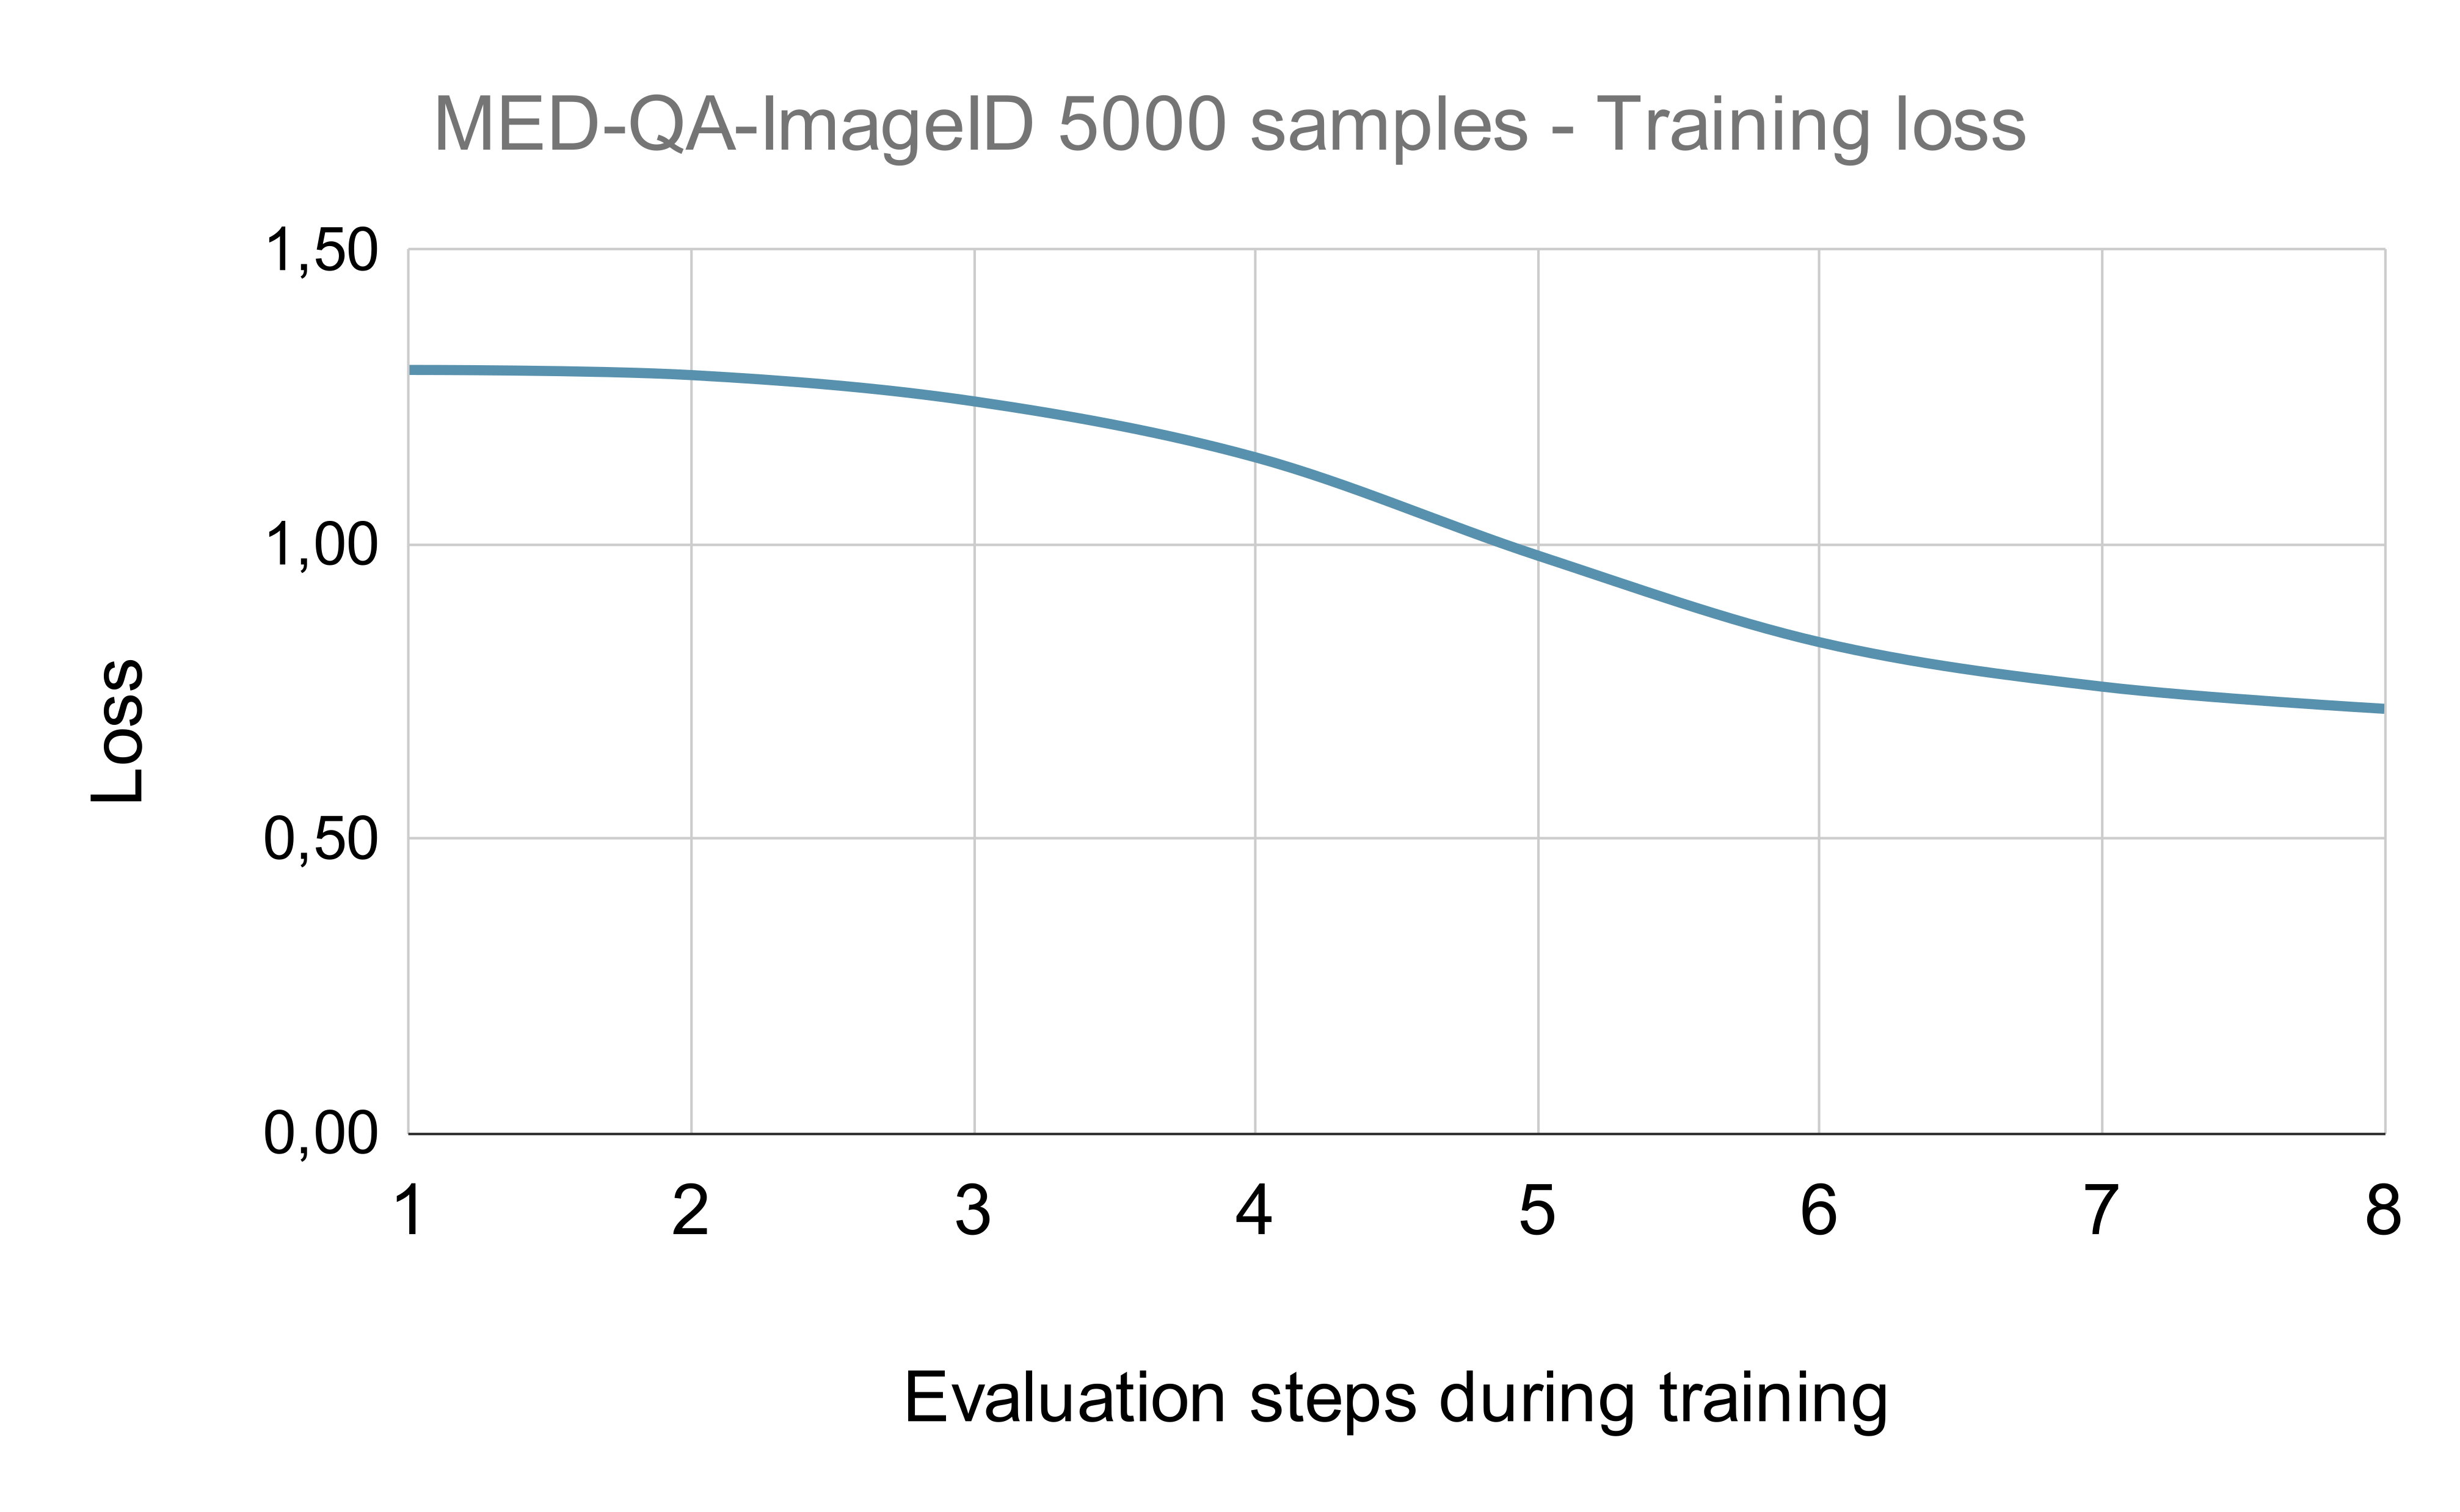
\includegraphics[width=\linewidth]{images/MED-QA-ImageID_5000_samples-Training_loss.png}
        \caption{Graph over training loss for initial test.}
        \label{fig:MED-QA-ImageID_5000_samples-Training_loss}
    \end{figure} 


    \paragraph{Analysis\\}
    
    It is helpful to analyze the dataset used in training to investigate why the model often answers with "Not relevant".
    When analyzing the correct answers in the dataset, as seen in Figure \ref{fig:ImageCLEFmed-MEDVQA-GI-2023_answer_label_balance}, the dataset is unbalanced and has a majority of correct answers being "Not relevant". This dataset can be balanced by either over-sample the other classes, or under-sample the abundant class, making the model learn "Not Relevant" is not the best answer in 21,7\% of all questions.
    Going further in future experiments the dataset will be a modified version of the original dataset, with the class "Not relevant" being under-sampled.
    
    


    \begin{figure}[htb]
        \centerline{
        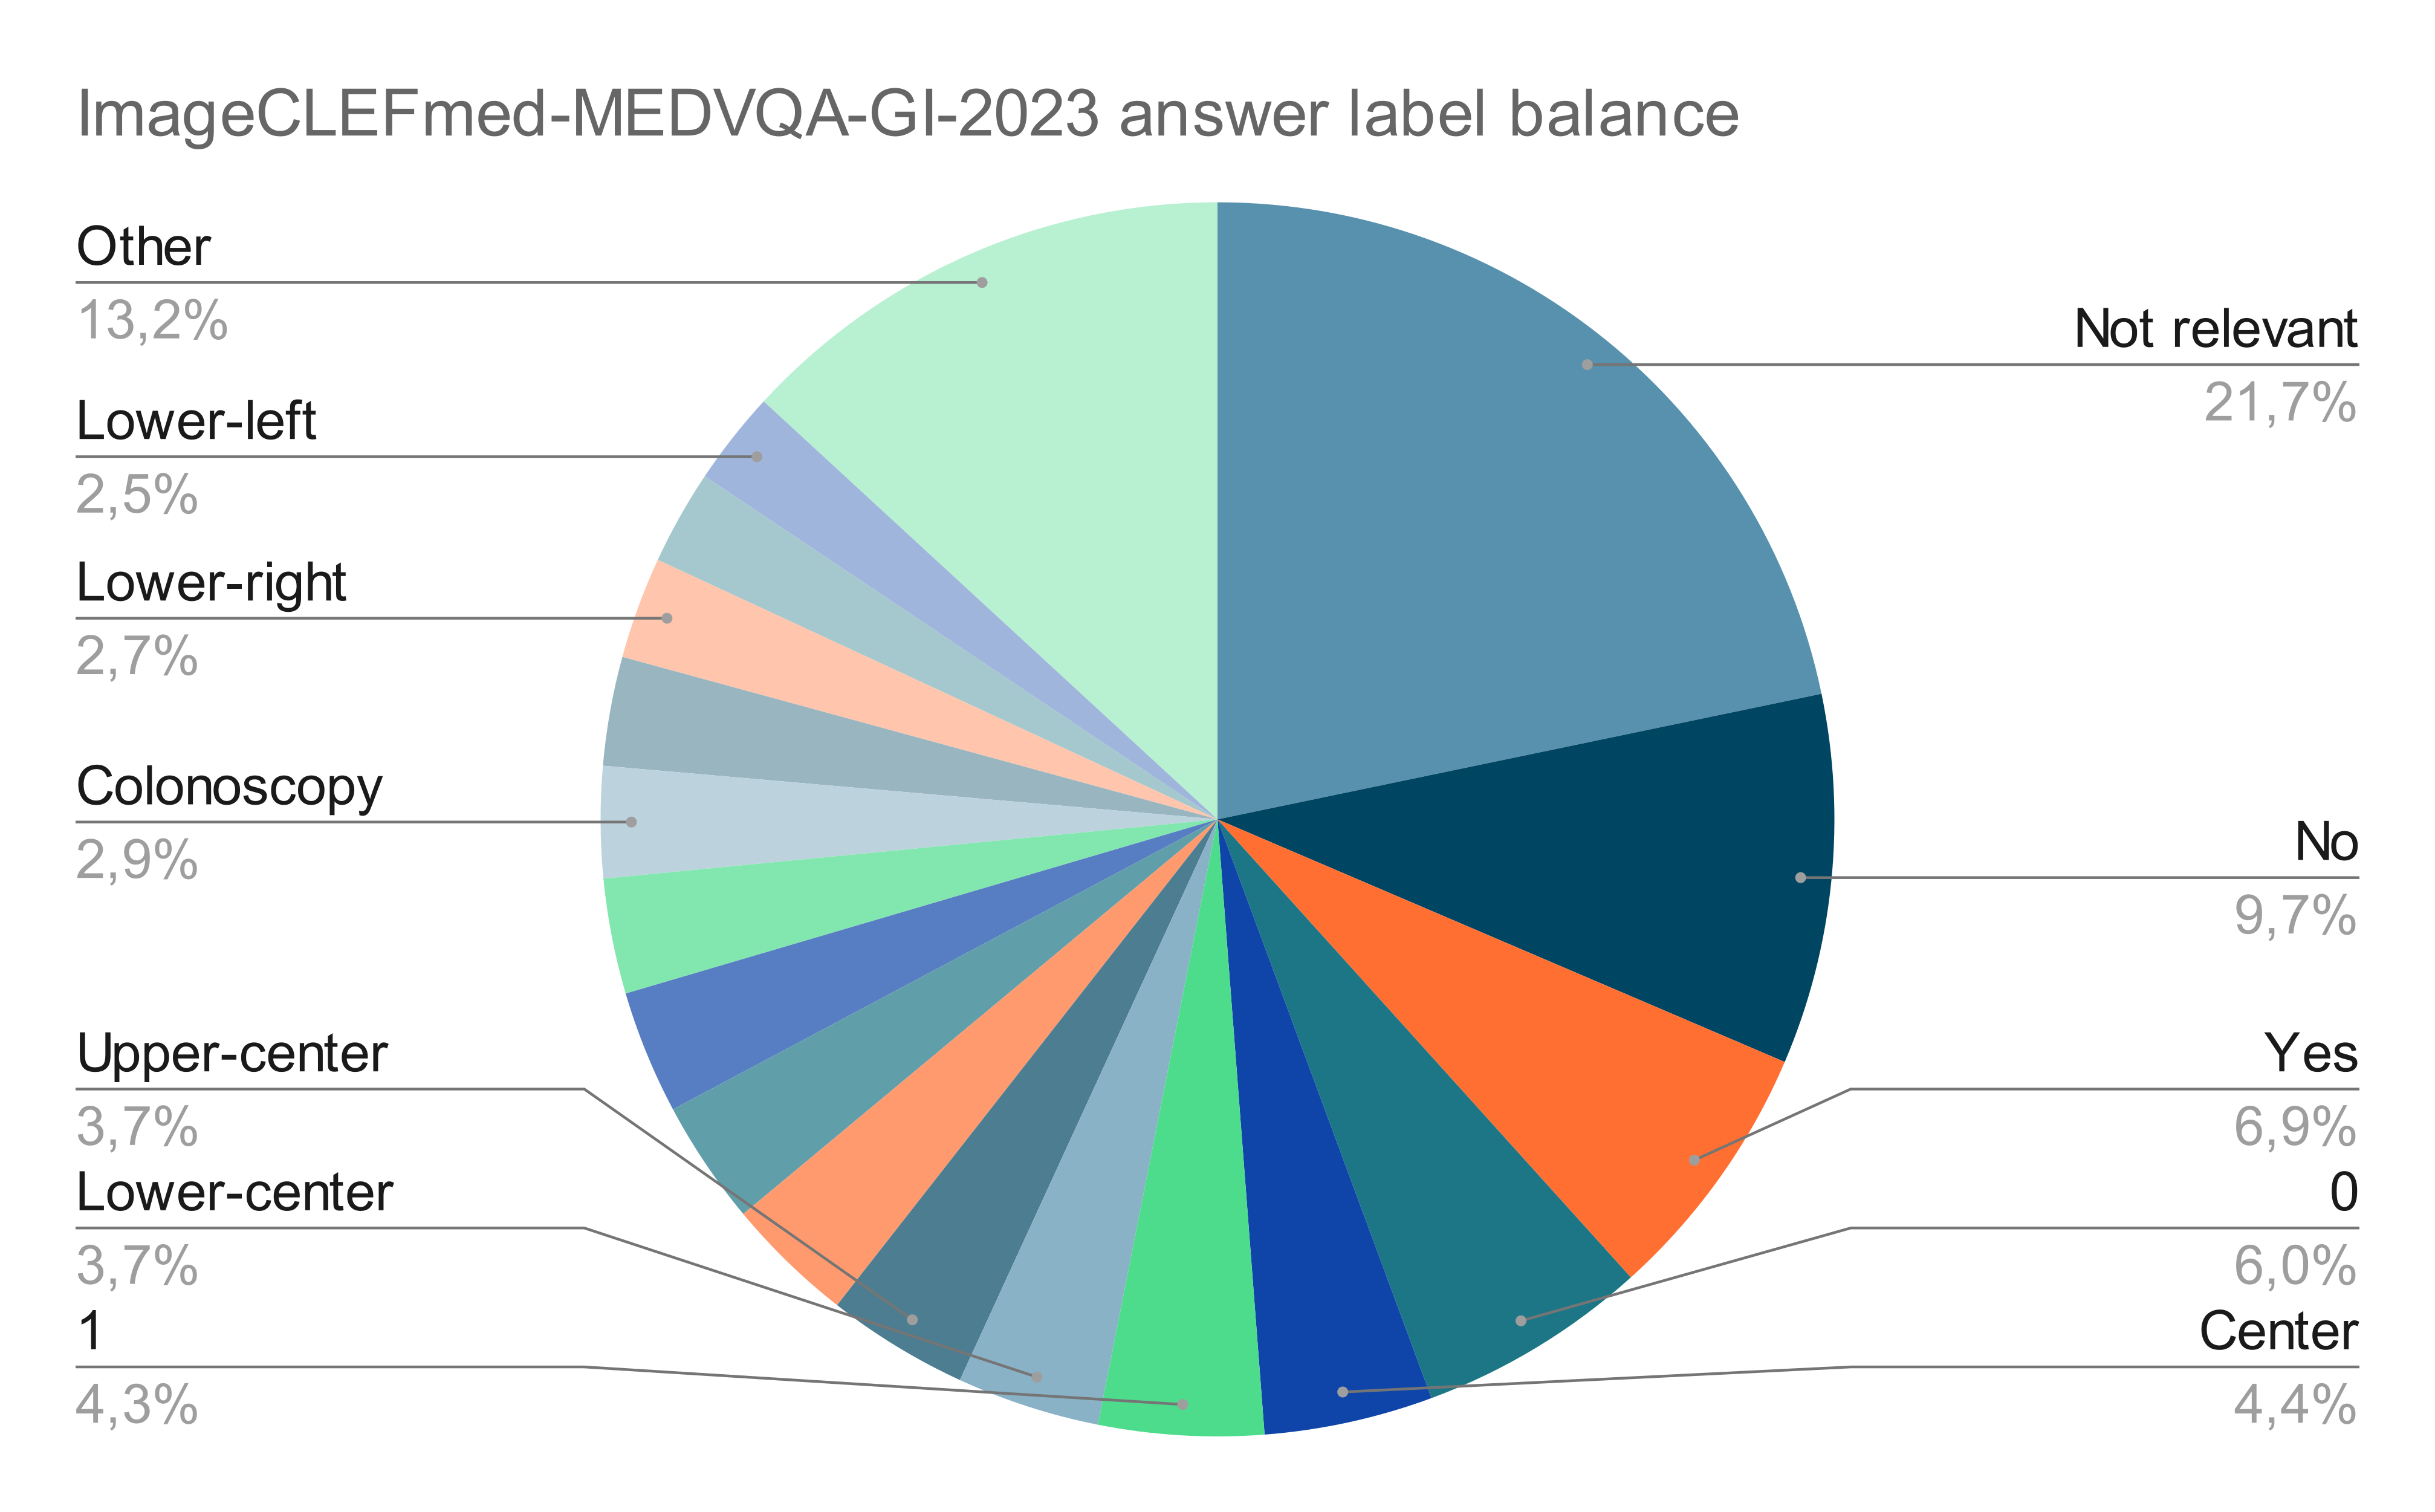
\includegraphics[width=17cm]{images/ImageCLEFmed-MEDVQA-GI-2023_answer_label_balance.png}}
        \caption{Overview of the answer label balance in the ImageCLEFmed-MEDVQA-GI-2023 dataset. Note that the category "segmentation" is already removed from the dataset due to not being relevant for this task at this stage. The category "Other" is a collection of 46 smaller labels.}
        \label{fig:ImageCLEFmed-MEDVQA-GI-2023_answer_label_balance}
    \end{figure} 


    \subsection{20'000 samples and 3 epochs}

    To address the issue where the model most often predicts the answer "Not relevant", a modified dataset, where this class is removed is used. The choice to remove this class completely is based on making the model see more relevant data. By removing this class, the 20'000 samples will contain more question-answer samples that are relevant to this classification problem. While it would be interesting to train the model on much more data, the time and the computing cost for this thesis would not justify the possible increase in a more generalized and nuanced model. This modification is also made to the evaluation dataset, which The resulting dataset used for training in this experiment contains 20'000 samples, and the class distribution can be seen in Figure \ref{fig:ImageCLEFmed-MEDVQA-GI-2023_answer_label_balance-modified}.

    The hyperparameters used are the same as in the previous experiment and can be seen in Table \ref{table:hyperparameters_5000}. The dataset used in this experiment contains four times more samples than in the previous experiment and the image feature extraction is still the top 100 features from the VGG16 model. Due to the similarities in the data samples, the hyperparameters can be kept the same, to see how the Alpaca model responds to a larger dataset.
    
    \begin{figure}[htb]
        \centerline{
        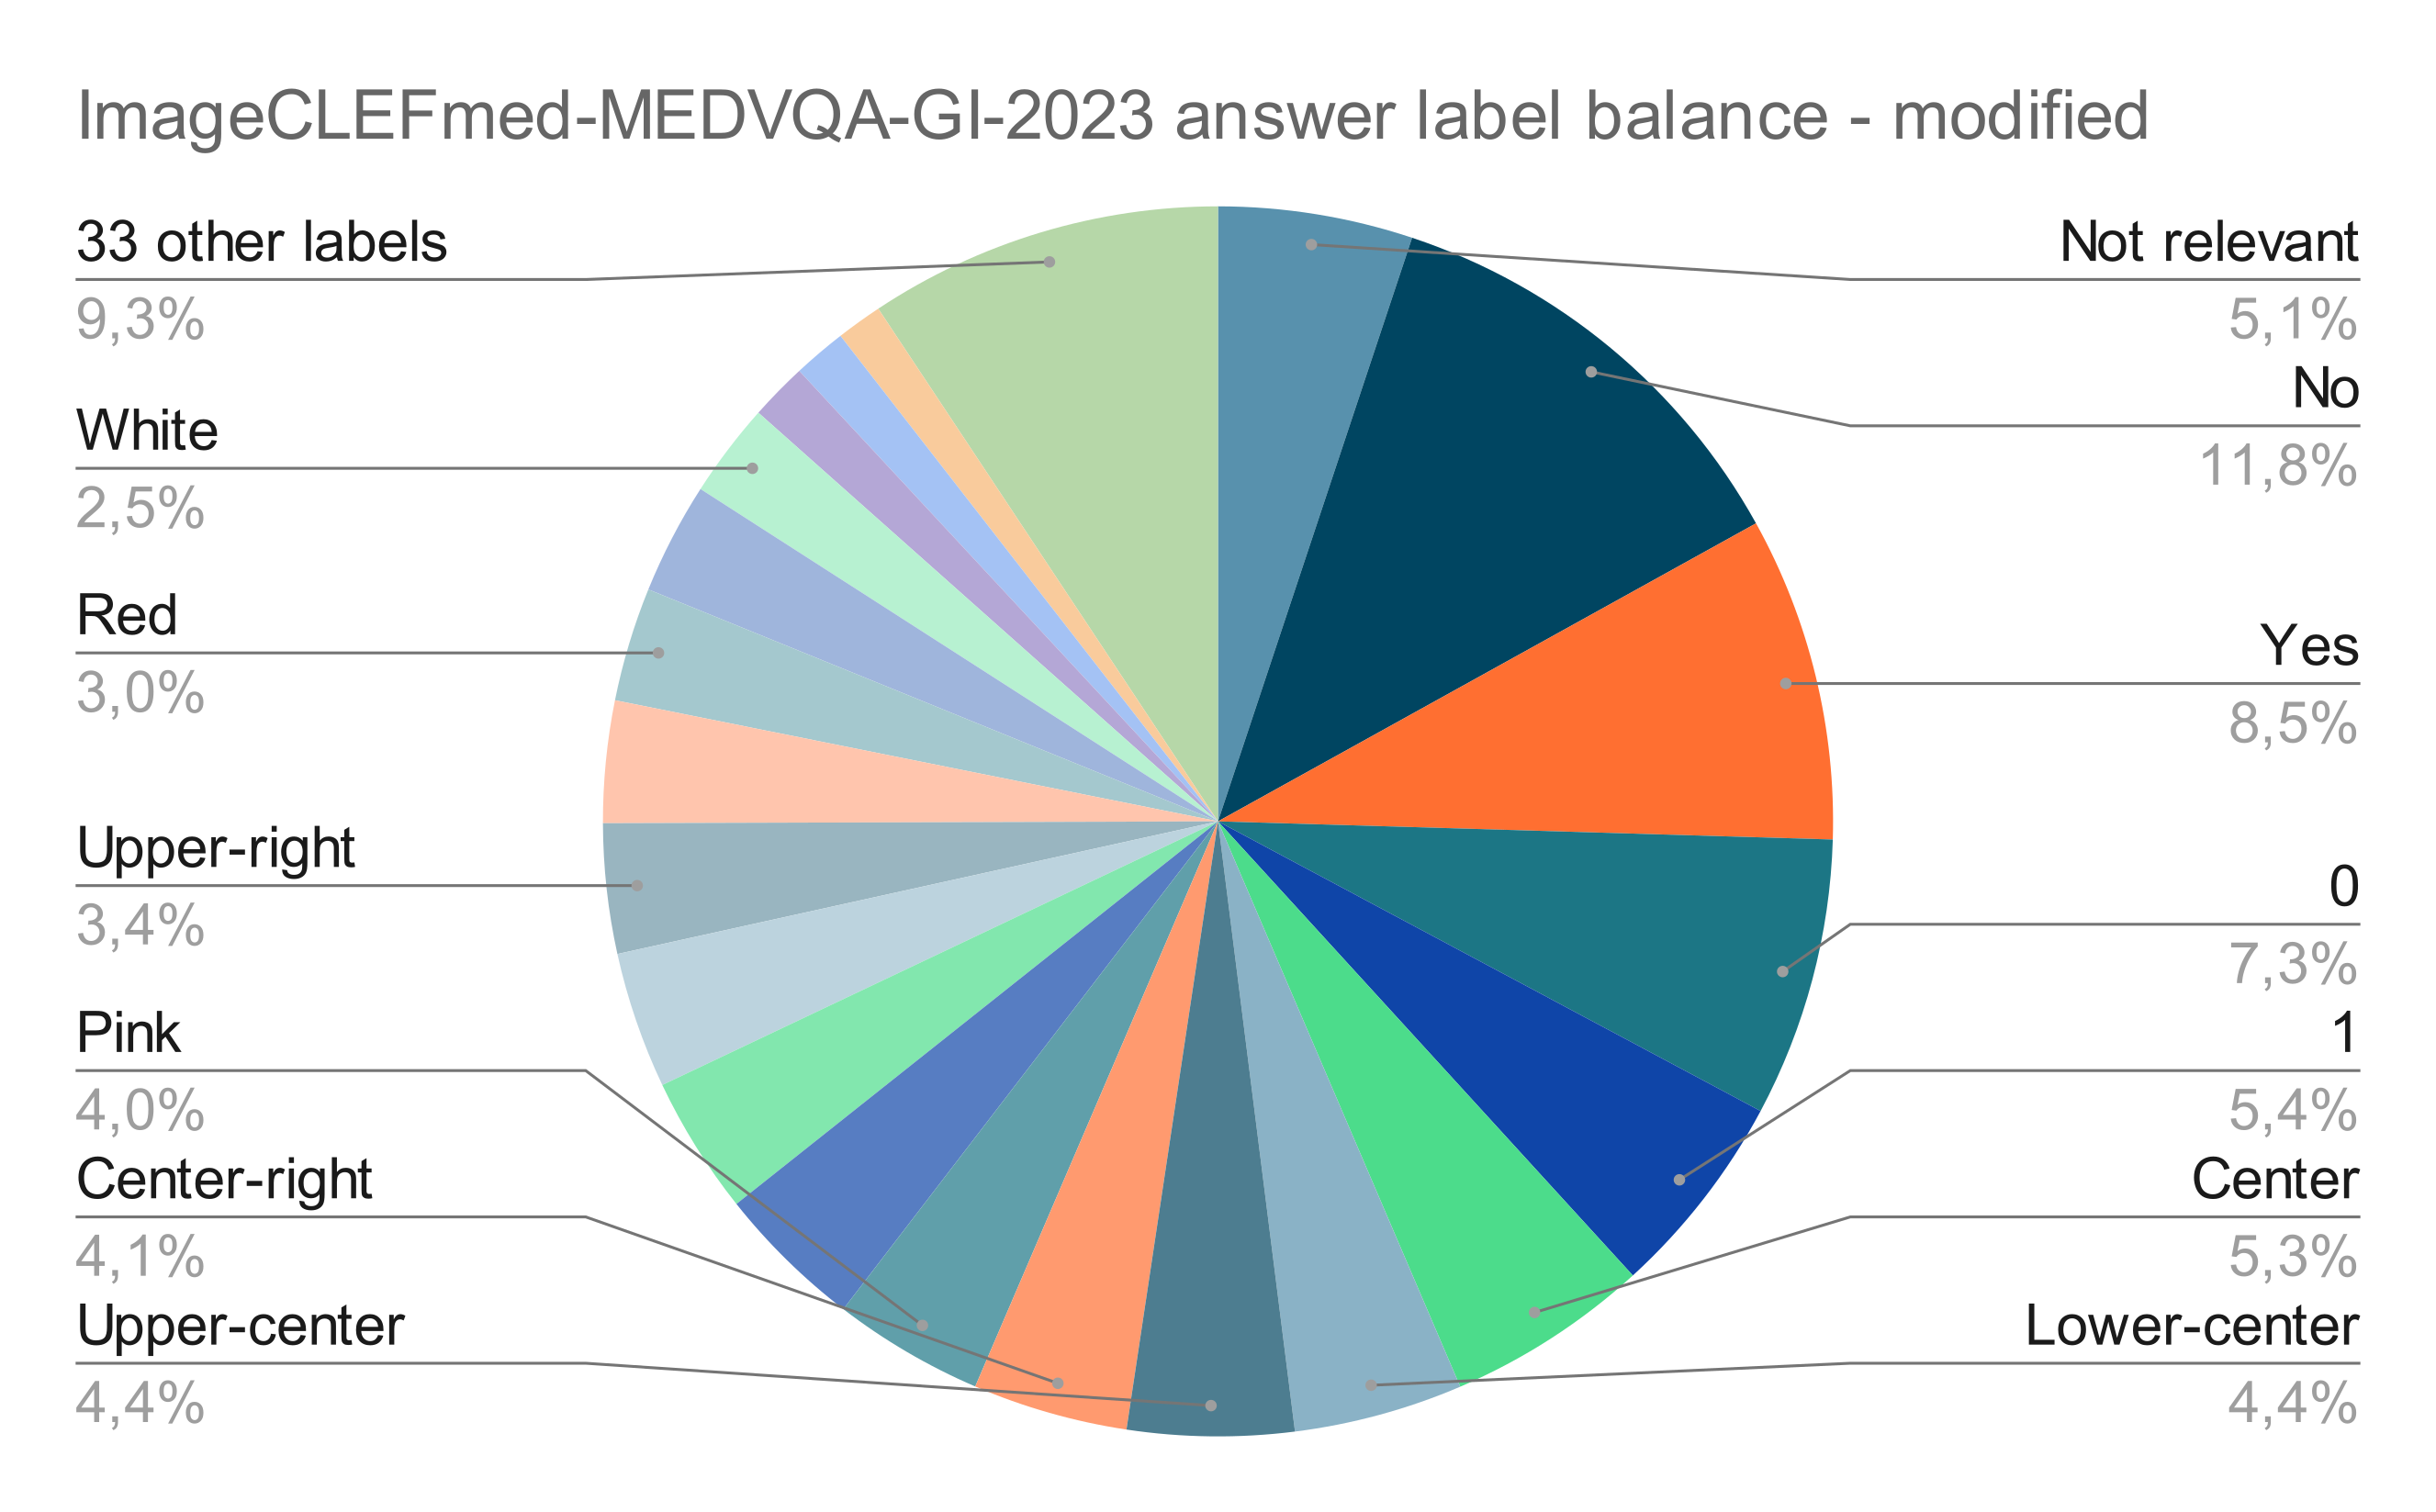
\includegraphics[width=17cm]{images/ImageCLEFmed-MEDVQA-GI-2023-answer-label-balance-modified.png}}
        \caption{Overview of the answer label distribution in the ImageCLEFmed-MEDVQA-GI-2023 dataset, modified with under-sampled class "Not relevant". The category "Other" is a collection of 33 smaller labels in the training data.}
        \label{fig:ImageCLEFmed-MEDVQA-GI-2023_answer_label_balance-modified}
    \end{figure} 

    \begin{center}
\begin{longtable}{|c|c|c|c|c|}
\caption{Classification Report on Test Set - Model trained on 20'000 question-answer pairs.} \label{tab:classification_report_20} \\

\hline \multicolumn{1}{|c|}{\textbf{Class}} & \multicolumn{1}{c|}{\textbf{Precision}} & \multicolumn{1}{c|}{\textbf{Recall}} & \multicolumn{1}{c|}{\textbf{F1-score}} & \multicolumn{1}{c|}{\textbf{Support}}\\ \hline 
\endfirsthead

\multicolumn{3}{c}%
{{\bfseries \tablename\ \thetable{} -- continued from previous page}} \\
\hline \multicolumn{1}{|c|}{\textbf{Class}} & \multicolumn{1}{c|}{\textbf{Precision}} & \multicolumn{1}{c|}{\textbf{Recall}} & \multicolumn{1}{c|}{\textbf{F1-score}} & \multicolumn{1}{c|}{\textbf{Support}}\\ \hline 
\endhead

\hline \multicolumn{5}{|r|}{{Continued on next page}} \\ \hline
\endfoot

\hline \hline
\endlastfoot




0 & 0.54 & 0.92 & 0.68 & 1551 \\
1 & 0.52 & 0.16 & 0.25 & 1132 \\
11-20mm & 0.00 & 0.00 & 0.00 & 97 \\
2 & 0.00 & 0.00 & 0.00 & 306 \\
3 & 0.00 & 0.00 & 0.00 & 13 \\
4 & 0.00 & 0.00 & 0.00 & 2 \\
5 & 0.00 & 0.00 & 0.00 & 2 \\
5-10mm & 0.00 & 0.00 & 0.00 & 100 \\
< 5mm & 0.00 & 0.00 & 0.00 & 55 \\
>20mm & 0.00 & 0.00 & 0.00 & 71 \\
Biopsy forceps & 0.00 & 0.00 & 0.00 & 43 \\
Black & 0.00 & 0.00 & 0.00 & 9 \\
Blue & 0.00 & 0.00 & 0.00 & 4 \\
Brown & 0.00 & 0.00 & 0.00 & 10 \\
Cecum & 0.00 & 0.00 & 0.00 & 33 \\
Center & 0.00 & 0.00 & 0.00 & 1121 \\
Center-left & 0.10 & 0.14 & 0.12 & 831 \\
Center-right & 0.11 & 0.43 & 0.17 & 861 \\
Colonoscopy & 0.98 & 0.05 & 0.10 & 761 \\
Gastroscopy & 0.00 & 0.00 & 0.00 & 242 \\
Green & 0.00 & 0.00 & 0.00 & 3 \\
Grey & 0.00 & 0.00 & 0.00 & 16 \\
Ileum & 0.00 & 0.00 & 0.00 & 2 \\
Injection needle & 0.00 & 0.00 & 0.00 & 1 \\
Lower-center & 0.00 & 0.00 & 0.00 & 938 \\
Lower-left & 0.00 & 0.00 & 0.00 & 616 \\
Lower-right & 0.11 & 0.06 & 0.08 & 769 \\
Metal clip & 0.00 & 0.00 & 0.00 & 11 \\
No & 0.66 & 0.46 & 0.54 & 2505 \\
Oesophagitis & 1.00 & 0.00 & 0.01 & 240 \\
Orange & 0.00 & 0.00 & 0.00 & 16 \\
Pale Pink & 0.00 & 0.00 & 0.00 & 1 \\
Paris iia & 0.00 & 0.00 & 0.00 & 95 \\
Paris ip & 0.00 & 0.00 & 0.00 & 101 \\
Paris is & 0.00 & 0.00 & 0.00 & 125 \\
Pink & 0.38 & 0.04 & 0.07 & 819 \\
Polyp & 0.25 & 0.96 & 0.39 & 311 \\
Polyp snare & 0.00 & 0.00 & 0.00 & 30 \\
Purple & 0.00 & 0.00 & 0.00 & 1 \\
Pylorus & 0.00 & 0.00 & 0.00 & 1 \\
Red & 0.29 & 0.27 & 0.28 & 629 \\
Tube & 0.00 & 0.00 & 0.00 & 218 \\
Ulcerative colitis & 0.00 & 0.00 & 0.00 & 250 \\
Upper-center & 0.00 & 0.00 & 0.00 & 944 \\
Upper-left & 0.00 & 0.00 & 0.00 & 764 \\
Upper-right & 0.11 & 0.38 & 0.16 & 729 \\
White & 0.00 & 0.00 & 0.00 & 520 \\
Yellow & 0.02 & 0.06 & 0.03 & 79 \\
Yes & 0.59 & 0.98 & 0.74 & 1778 \\
Z-line & 0.00 & 0.00 & 0.00 & 220 \\
Brown & 0.00 & 0.00 & 0.00 & 4 \\
Grey & 0.00 & 0.00 & 0.00 & 7 \\
Purple & 0.00 & 0.00 & 0.00 & 3 \\
\hline
Accuracy &  &  & 0.29 & 20000 \\
Macro average & 0.09 & 0.08 & 0.06 & 20000 \\
Weighted average & 0.30 & 0.29 & 0.24 & 20000 \\

\end{longtable}
\end{center}



% DISCUSSION:
\label{4_discussion}

\section{Discussion}

    % Using more modern CV-methods, like YOLO, instead of gradients of CNN.


% SUMMARY: